% !TeX encoding = UTF-8
% !TeX program = xelatex
% !TeX spellcheck = en_US

\documentclass[degree=project,degree-type=project,cjk-font=noto]{thuthesis}
% 著者-出版年制
\usepackage[sort]{natbib}
\bibliographystyle{thuthesis-author-year}
\usepackage{mathtools}
\usepackage{tikz}
\usetikzlibrary{shapes,arrows}
\usepackage[autosize]{dot2texi}
% Syntax Highlighting in LaTeX, need pygments
% Must build with xelatex -shell-escape -enable-8bit-chars.
\usepackage{minted}
% https://tex.stackexchange.com/a/112573
\usepackage{tcolorbox}
\usepackage{etoolbox}
\BeforeBeginEnvironment{minted}{\begin{tcolorbox}}%
\AfterEndEnvironment{minted}{\end{tcolorbox}}%
% color for minted
\definecolor{friendlybg}{HTML}{f0f0f0}


% 论文基本配置,加载宏包等全局配置
\thusetup{
    output = electronic,
    title  = {推荐系统},
    author  = {肖文韬},
    studentid = {2020214245},
    major = {电子信息(计算机技术)},
    email = {xwt20@mails.tsinghua.edu.cn},
    course = {大数据分析(B)},
    include-spine = false,
}

\usepackage{float}
\graphicspath{{figures/}}


\begin{document}

% 封面
\maketitle

\frontmatter
\begin{abstract}
  推荐系统的数据来源的特点是多域(multi-field)数据,即数据由来源于许多不同域的特征组合而成(例如用户性别、年龄、浏览记录等)。
  这些多域数据的组合特征(combinatorial features)便是许多商业模式成功的必要条件。
  最近,许多深度模型被提出来从原始特征中学习低阶和高阶特征组合。
  点击率预测作为推荐系统中的一项重要任务,其目的是估计用户点击某项目的概率,对许多在线应用(如在线广告)至关重要。
  本文将探究以 xDeepFM 为代表的论文是如何解决点击率预测问题的。
  论文将首先对 xDeepFM 之前和之后的论文做一个简单的综述,然后对点击率预测问题进行形式化定义。
  接着,xDeepFM 以及后面提出的 AutoInt 和 FGCNN 的算法将被详细介绍。
  最后,本文将复现上述三个方法,并分析它们的实验结果。

  \thusetup{
    keywords = {推荐系统, 点击率预测,深度学习, xDeepFM, AutoInt, FGCNN},
	}
\end{abstract}

\begin{abstract*}
  The data sources of recommendation systems are characterized by multi-field data, i.e., the data consists of a combination of features from many different domains (e.g., user gender, age, browsing history, etc.).
  These combined features of multi-field data are necessary for the success of many business models.
  Recently, many deep models have been proposed to learn combinations of low- and high-order features from the original features.
  Click-through prediction, an important task in recommender systems, aims to estimate the probability that a user will click on an item and is crucial for many online applications such as online advertising.
  In this paper, we will explore how the click-through rate prediction problem is addressed in a paper represented by xDeepFM.
  The paper will first give a brief overview of the papers before and after xDeepFM, followed by a formal definition of the click-through rate prediction problem.
  Then, xDeepFM and the later proposed algorithms of AutoInt and FGCNN will be presented in detail.
  Finally, the paper will reproduce the above three methods and analyze their experimental results.

  % Use comma as seperator when inputting
  \thusetup{
    keywords* = {Recommendation System, click-through rate, deep learning, xDeepFM, AutoInt, FGCNN},
  }
\end{abstract*}


% 目录
\tableofcontents

% 插图和附表清单
\listoffiguresandtables
% \listoffigures           % 插图清单

% 正文部分
\mainmatter

\chapter{引言}

推荐系统是防止消费者过度选择的一道直观防线。
鉴于网络上信息的爆炸性增长,用户经常会被无数的商品、电影或餐馆所吸引。
因此,个性化是促进更好的用户体验的重要策略。
总而言之,这些系统在各种信息访问系统中一直扮演着重要和不可或缺的角色,以促进业务和促进决策过程,并在众多网络领域,如电子商务和/或媒体网站中普遍存在。

一般来说,推荐列表是基于用户偏好、物品特征、用户/物品过去的交互,以及其他一些附加信息,如时间(如序列感知推荐器)和空间(如POI)数据生成的。
根据输入数据的类型,推荐模型主要分为协同过滤、基于内容的推荐系统和混合推荐系统。

过去的几十年里,深度学习在计算机视觉和语音识别等许多应用领域取得了巨大的成功。由于深度学习能够解决许多复杂的任务,同时提供最先进的结果,学术界和工业界一直在竞相将深度学习应用到更广泛的应用中。
最近,深度学习极大地改变了推荐架构,并为提高推荐系统的性能(如召回率、精确率等)带来了更多机会。最近,基于深度学习的推荐系统的进展克服了传统模型的障碍,实现了高推荐质量,从而获得了极大的关注。深度学习能够有效地捕捉非线性和非平凡的用户/项目关系,并能将更复杂的抽象内容编纂成上层的数据表示。此外,它还能从丰富的可访问数据源(如上下文、文本和视觉信息)中捕捉到数据本身的复杂关系。

本文关注的重点是点击率预测 (click-through rate, CTR) ,作为推荐系统中的一项重要任务,其任务是估计用户点击推荐项目的概率。在很多推荐系统中,目标是最大化点击次数,因此可以通过估算CTR对返回给用户的项目进行排序;而在其他应用场景中,如在线广告,提高收益也很重要,因此可以将排序策略调整为所有候选项目的 CTR×bid,其中 "bid"(出价) 是指项目被用户点击后系统获得的收益。无论哪种情况,显然关键在于正确估计CTR。

CTR 数据有以下特点:

\begin{itemize}
  \item 数据按照域(field)来划分,每个域的特征是独立表示的。
  \item 数据含有离散型的域,也有连续型的域。一般离散型的域用独热(one-hot)向量表示,而连续型的数据可以离散化后再变为独热向量,也可以直接用连续值。
  \item 因为大量使用独热向量,所以特征维度非常高。
  \item 数据非常稀疏。
\end{itemize}

所以,CTR 的重点一般在于如何学习不同域之间的特征组合 (field interaction)。

\chapter{文献综述}

按照是否是基于深度学习,推荐系统可以分为传统方法和基于深度学习的方法。
对于传统方法,大致可以分为线性模型和因式分解机模型。
同时,基于深度学习的方法按照出现的时间又可以分为 xDeepFM 及以前的方法,以及 xDeepFM 以后的方法。

\section{经典推荐系统}

\subsection{线性模型}

对于互联网规模的推荐系统,其输入特征一般是离散、连续混杂的高维数据。
线性模型,例如 \cite{tfrl} 提出的 FTRL 逻辑回归,因其易于管理、维护和部署,在工业界被广泛使用。
不过这些线性模型有一个严重的缺点:它们无法学习特征组合,它们只能用于解决线性可分或近似线性可分的问题。
这意味着数据科学家必须花费大量的时间进行人工的特征组合来获得更好的结果。
并且,很多特征组合很难被手工设计出来,所以也有一些研究者采用加速决策树来帮助进行特征转换(\cite{ctr_bing})。

\subsection{因式分解机模型}

线性模型的一个主要缺点就是无法泛化到训练集中没有见过的特征组合。
以 \cite{fm} 提出的因式分解机(Factorization Machines, FM)为代表的方法通过将每一个域特征嵌入(embedding)为一个低维隐向量中来解决这个问题。
作为推荐系统领域最热门的基于模型的协同过滤方法,\cite{mf} 提出的矩阵因式分解(Matrix factorization, MF)可以视作一种只考虑 ID 作为特征的特殊的 FM。
MF 的推荐结果通过两个隐向量的乘积得出,也就是说它并不需要在数据集中提供用户和物品的同现关系(co-occurrence)。
另一方面,对于许多推荐系统来说,只有用户的观看历史和浏览活动等隐性反馈数据集。因此研究者将因式分解模型扩展到隐性反馈的贝叶斯个性化排名(BPR)框架中(\cite{vbpr})。

FM 使用隐向量的内积作为特征组合,解决了线性模型无法提取特征组合的问题。
但是实际使用中因为计算复杂度较大,一般也就只能最多计算 2 阶特征组合。
后来,FM 的一种变体 FFM (\cite{ffm}) 提出了域(field)的概念,把相同性质的特征放在同一个域(例如很多个表示日期的特征)。
同一个特征与不同域的特征进行特征组合的时候,会使用不同的隐向量。

\section{基于深度学习的方法}

\subsection{xDeepFM 及以前的方法}

xDeepFM 及有关的论文主要思路为:使用深度学习来学习(高阶)特征组合。
按照出现时间排序,主要有以下方法:

随着深度学习的成功,\cite{fnn} 提出的 FNN 作为将 DNN 应用于 FM 的早期尝试,主要思路就是使用预训练的 FM 的输出隐向量来作为 DNN 的输入,对 DNN 进行训练。
FNN 可以理解为潜入层固定的 embedding + MLP 结构。
优点是可以学习更高阶的特征组合,并且因为采用预训练 FM,DNN 模型的收敛速度快一点。
缺点有:

\begin{enumerate}
  \item 性能受预训练 FM 影响
  \item 预训练 FM 加大了计算复杂度
  \item 只能学习高阶特征组合
\end{enumerate}

\cite{pnn} 提出的 PNN 相比之 FNN,在 embedding 和 DNN 之间加入了一层 product layer。
PNN 的思想是认为 CTR 场景中特征组合更多的是“且”操作(也就是乘法),而不是“或”操作(加法),因而加入乘积层。
同时,根据 product 的不同(内积,外积,混用),还可以分为 IPNN,OPNN和PNN*三种。
PNN 的缺点有:
\begin{enumerate}
  \item 乘积计算复杂度较高
  \item 和 FNN 类似,只能学习高阶特征,缺乏一阶和二阶特征
\end{enumerate}

总结上述 FNN 和 PNN 的缺点,来自 Google 的 \cite{deep_wide} 提出了 Deep \& Wide 组合了深度模型学习到的高阶特征(Deep)和传统线性模型的低阶特征 (Wide)。
显著地提高了模型的性能。
不过缺点有:

\begin{enumerate}
  \item 低阶特征需要基于领域知识的特征工程
  \item 无法端到端训练
\end{enumerate}

受到 \cite{resnet} 提出的残差网络思想的启发,\cite{deep_cross} 提出了 DeepCross 将深度残差网络引入到 CTR 中。
对比之前的论文,Deep Cross 对 MLP 部分添加残差连接,同时 MLP 可以更加深。
同样受残差网络影响的,还有 \cite{dcn} 提出的 Deep \& Cross (DCN),改论文主要是解决之前提出的 Deep \& Wide 中 Wide 部分需要专家经验的特征工程的问题。
DCN 将 Wide 部分用 Cross Layer 来代替,Cross Layer 可以自动构造有限高阶特征组合。
采用残差连接,$l + 1$ 层的输出为 $x_{l+1} = x_0 x_l^T w_l + b_l + x_l$。
虽然这个公式看起来跟 MLP 挺像的,不过如果展开里面的递推(残差)项后,我能发现,$l + 1 $ 层的输出结果正好是 $l + 2$ 阶叉乘的结果。
Cross 部分因为参数共享的设计,模型参数与输入维度为线性关系,相比于 DNN 节约很多内存。
而且因为 Cross 部分也是神经网络,所以可以进行端到端训练。
不过缺点有:

\begin{enumerate}
  \item Cross Layer 只考虑了自动叉乘
  \item Cross 和 DNN 部分的能力不匹配,在大规模生产数据上尤为明显
\end{enumerate}

同样的,\cite{deepfm} 提出的 DeepFM 在 Wide \& Deep 基础上,对其 Wide 部分进行改进,将 Wide 部分换为 FM。
FM 用于提取低阶特征组合,Deep 部分用于提取高阶特征组合。
FM 和 Deep 部分共享特征嵌入,这样训练的也更加快一点。
FM 部分由一个加法单元和多个内积单元组成。
这样,DeepFM 有以下优点:

\begin{enumerate}
  \item 端到端训练, 不需要基于专家经验的特征工程
  \item 相对于 PNN,训练效率高
\end{enumerate}

值得注意的是,实际应用的时候我会需要许多同领域历史数据,例如某个用户浏览了 10 个商家,常规的做法会将这些同领域的数据直接求和得到一个嵌入向量。
但是其实这 10 个商家可能只有一两个跟要被预测的目标广告相关。
受到 \cite{attention} 提出的注意力机制启发,\cite{din} 提出了 Deep Interest Network (DIN)。
它的思想就是对于同域的历史数据,DIN 会对其分配不同的权重(注意力)来求和。

前面提出的这么多的基于 DNN 的模型,DNN 学习到的特征组合都是隐式的,也就是说我无法知道模型学出来的特征组合是几阶的以及与哪几个域的特征有关。
并且 DNN 中全连接层的运算都是 bit-wise 而不是 field-wise。
也就是说,同一个 field 的 embedding 里面不同位之间还要相互运算,这显然对特征组合来说是没有必要的。
同时,Deep \& Cross 和 DeepFM 的成功说明,显式的特征组合是有必要的。
\cite{xdeepfm} 提出的 xDeepFM 基于 DCN 和 DeepFM,将 Cross 层用 CIN 替代。
CIN 可以学习 vector-wise 的显示特征组合,并且 xDeepFM 的作者认为 DCN 的 Cross 只能学习 $x_0$ 的标量倍数,学习特征组合能力有限,而 CIN 的学习能力更强。
CIN 的结构类似于 CNN 和 RNN,对于 $k$ 阶多项式的估计,只需要 $\mathcal{O(km^3)}$ 的时间复杂度。
总的来说,xDeepFM 的缺点有:

\begin{enumerate}
  \item CIN 的复杂度仍然太高
\end{enumerate}

\subsection{xDeepFM 以后的方法}
\label{sec:after_xeepfm}

随着采用自注意力机制的 Transformer(\cite{self_attention})在 NLP 领域的成功应用,\cite{autoint} 使用自注意力网络来学习特征组合,并且在 CTR 应用上取得了成功。
特征组合层采用类似于 Transformer 的多头自注意力机制,不同域的 embedding 作为一个单元组成输入特征序列。
这样每一个特征都能与其他特征进行组合,并且按照注意力机制对不同特征的相关性进行打分,以此来学习高阶特征组合。
残差连接也被加入到网络中,这样可以保证网络更加深,学习到更多的特征组合。
同时,注意力机制也为不同特征之间的相关关系提供了很好的可视化解释。
缺点:

\begin{enumerate}
  \item 参数规模比较大
  \item 时间复杂度较大
\end{enumerate}

另一方面,FGCNN (\cite{fgcnn})为了解决特征的问题,提出使用 CNN 来学习新的特征与原始输入拼接在一起作为 CTR 模型的输入。
不过因为我知道输入数据不同域之间是没有顺序可言的,也就是说,特征按照不同顺序摆放对最终结果影响不大。
FGCNN 使用 CNN 来学习输入特征的局部特征,但是因为输入特征没有顺序可言,所以论文提出重组层(其实就是全连接层)来学习全局特征。
值得一提的是,FGCNN 只是特征生成器,得到的新特征还要继续交给 CTR 模型去预测结果,说白了就是为已有的 CTR 模型做数据增强。
缺点:

\begin{enumerate}
  \item 结果依赖 CTR 分类器(不是FGCNN 负责的),所以不是端到端的模型
  \item 计算复杂度很大,因为复杂度相当于是 FGCNN 的部分再加上分类器的那部分
  \item CNN 在 CTR 上的应用的说服力不够强
\end{enumerate}

为了解决 DCN 的 Cross 能力较弱,并且解决实际大规模应用时的问题。
\cite{dcn_v2} 提出了 DCN v2 在更低的计算开销的情况下取得了最先进的结果。
并且它在 Google 的多个推荐系统的线上和线下测试中都取得了很好的结果。
DCN-V2的核心是交叉层,它继承了DCN的简单结构的交叉网络,然而在学习显式和有界度的交叉特征时,表现力明显增强。
因为模型学习到的矩阵的低秩性质,DCN v2 提出利用低秩技术来逼近子空间中的特征组合,以实现更好的性能和延迟权衡。
此外,论文还提出了一种基于Mixture-of-Expert架构(\cite{mix_experts})的技术,以进一步将矩阵分解成多个更小的子空间。
然后通过门控机制对这些子空间进行聚合。


为了解决深度神经网络计算复杂度的问题,\cite{deeplight} 提出的 DeepLight 提出许多技巧来加速 CTR 的预测。
最终实验表明,DeepLight 在不损失任何预测精度的前提下,在 Criteo 数据集和 Avazu 数据集上分别取得了 46 和 27 倍的模型推导速度提升。
这有助于将模型部署到生产环境中。
DeepLight 加速 CTR 速度主要来自于以下三个方面:

\begin{enumerate}
  \item 通过显示地搜索浅层组件中的信息特征相互作用来加速模型推理
  \item 修剪DNN组件中层间的冗余参数
  \item 修剪稠密嵌入向量,使它们在嵌入矩阵中变得稀疏
\end{enumerate}


\chapter{算法总结}

\section{任务定义}

对于模型输入,我将用户档案和项目属性表示为一个稀疏矩阵,也就是将所有域特征在一起:

\begin{equation}
  \symbf{x} = [\symbf{x}_1; \symbf{x}_2; \cdots; \symbf{x}_M]
\end{equation}
其中共有 $M$ 个域,域特征 $\symbf{x}_i$ 可以是类别数据的独热向量,也可以是连续数据的标量值(长度为 $1$ 的向量)。

因为输入 $\bm{x}$ 是一个非常稀疏且维度巨大的向量,所以在 CTR 领域经常会使用嵌入技术,来将域特征嵌入为一个维度小很多的向量。
简单来说,嵌入就可以理解为左乘一个矩阵, 对域特征独热向量 $\bm{x}_i$ 的嵌入有:

\begin{equation}
  \bm{e}_i = \bm{V}_i \bm{x}_i
\end{equation}

如果对于同一个域有多个数据,例如一个人喜欢看的电影可能有动作、爱情和喜剧三种。
这样的话会产生三个同域的独热矩阵,为了计算他们的嵌入,我只需要把它们加起来 $\bm{x}_i$,然后:

\begin{equation}
  \bm{e}_i = \frac{1}{q} \bm{V}_i \bm{x}_i
\end{equation}
其中 $q$ 为这些同域特征的数量。

同样的,为了把标量连续实数值变为嵌入向量,我可以乘一个向量:

\begin{equation}
  \bm{e}_m = \bm{v}_m x_m
\end{equation}


CTR 的任务就是给定用户和项目数据 $\symbf{x}$,模型 $f: \mathbb{R}^n \rightarrow \{0, 1\}$ 需要预测该用户针对该项目是否会点击(二分类):

\begin{equation}
  \hat{y} = f(\symbf{x})
\end{equation}

一般来说嵌入层就是模型的第一层。
当然这个模型输出也可以是一个概率值。
这个模型既可以是传统方法,例如线性模型 $f(\symbf{x}) = \sigma(\symbf{w}^T \symbf{x} + b)$, 其中 $\sigma(\cdot)$ 是 sigmoid 函数。
当然这样的模型肯定是太简单了,就像前面所说的那样,我可以使用深度神经网络来(显式或隐式地)学习高阶、低阶特征交互,甚至是新特征。
这样能够在更大的假设空间中学习到更加适合的特征表示,找到人工很难甚至无法找到的发挥实际用处的特征组合。

对于神经网络,我一般使用交叉墒损失函数(其实就是负对数似然)作为目标函数:

\begin{equation} \label{eq:loss}
  \mathcal{L} = - \frac{1}{N} \sum_{i=1}^N y_i \log \hat{y}_i + (1 - y_i) \log (1 - \hat{y_i})
\end{equation}
其中 $N$ 是数据集中的样本数量。

当然,为了避免模型过拟合,我一般会设置一个正则化项:

\begin{equation}
  \mathcal{J} = \mathcal{L} + \lambda \lVert \Theta \rVert
\end{equation}
其中 $\lambda$ 正则化项的系数,$\lVert \cdot \rVert$ 是某中范数,$\Theta$ 是模型的参数。

\section{xDeepFM 模型}

假定嵌入层的输出为 $X^0 \in \mathbb{R}^{M \times D}$,$X^0_{i,*} = \bm{e}_i$, 也就是说嵌入维度为 $D$。
xDeepFM 主要由 CIN 和 DNN 两部分组成。
CIN 网络由很多一模一样的网络层堆叠而成,对于第 $k$ 层,其输入 $X^{k-1} \in \mathbb{R}^{H_{k-1} \times D}$,输出 $X^k \in \mathbb{R}^{H_k}$ 可以理解为通道数为 $D$ 的 1D CNN 输出特征图:

\begin{equation}
  X^k_{h,*} = \sum_{i=1}^{H_{k-1}} \sum_{j=1}^{M} W_{ij}^{k,h}(X_{i,*}^{k-1} \odot X_{j,*}^0)
\end{equation}
其中 $\odot$ 表示 Hadamard 乘(也就是逐位乘法), 参数 $W_{ij}^{k,h} \in \mathbb{R}^{H_k \times M}$。

对于深度为 $T$ 的 CIN 的输出 $\bm{p}^+$,可以看成是对每一层的输出特征图进行 $1\times 1$ 的累加池化(sum pool):

\begin{align}
  p_i^k &= \sum_{j=1}^D X_{i,j}^k, i \in [1, H_k] \\
  \bm{p}^k &= [p_1^k; \cdots, p_{H_k}^k] \\
  \bm{p}^+ &= [\bm{p}^1; \cdots; \bm{p}^T]
\end{align}

DNN 部分就是简单的 MLP,不再赘述。
此外,xDeepFM 还有一个线性层。
最终的 xDeepFM 表示为:

\begin{equation}
  \hat{y} = \sigma(\bm{w}_L^T \bm{a} + \bm{w}_D^T x^k_{dnn} + \bm{w}_C^T \bm{p}^+ + b)
\end{equation}
其中 $\bm{a}, \bm{x}^k_{dnn}$ 分别表示原始特征,$k$ 层 DNN 的输出。

\section{AutoInt 模型}
\label{sec:autoint}

AutoInt 除了第一层为嵌入层之外,核心就是采用了多层特征组合层,其实特征组合层就是多头注意力的输出。
定义嵌入层输出为 $\bm{e} \in \mathbb{M \times D}$。
对于第 $k$ 层特征组合层的第 $h$ 头(head),输入为 $\bm{e} \in \mathbb{R}^{M \times d}$, 输出 $\tilde{\bm{e}} \in \mathbb{R}^{M \times d^\prime}$:

\begin{align}
  \alpha_{m,k}^{(h)} &= \frac{\exp(\phi^{(h)}(\bm{e}_m, \bm{e}_k))}{\sum_{l=1}^M \exp(\phi^{(h)}(\bm{e}_m, \bm{e}_l))} \\
  \phi^{(h)}(\bm{e}_m, \bm{e}_k) &= \langle W_Q^{(h)} \bm{e}_m, W_K^{(h)} \bm{e}_k\rangle \\
  \tilde{\bm{e}}_m^{(h)} &= \sum_{k=1}^M \alpha_{m,k}^{(h)} (W_V^{(h)} \bm{e}_k) \\
\end{align}

该层(总共 $H$ 头)的输出就是将这些头的输出拼接在一起:

\begin{equation}
  \tilde{\bm{e}} = \tilde{\bm{e}}^{(1)} \oplus \cdots \oplus \tilde{\bm{e}}^{(H)}
\end{equation}

这样,多层特征组合层的输出还要与最开始的嵌入表示残差连接起来:

\begin{equation}
  \bm{e}^{R}_m = \text{ReLU}(\tilde{\bm{e}}_m + W_R \bm{e}_m)
\end{equation}

最后整个 AutoInt 的输出为:

\begin{equation}
  \hat{y} = \sigma(\bm{w}^T \bm{e}^R + b)
\end{equation}

\section{FGCNN 模型}
\label{sec:fgcnn}

\begin{figure}[h]
\centering%
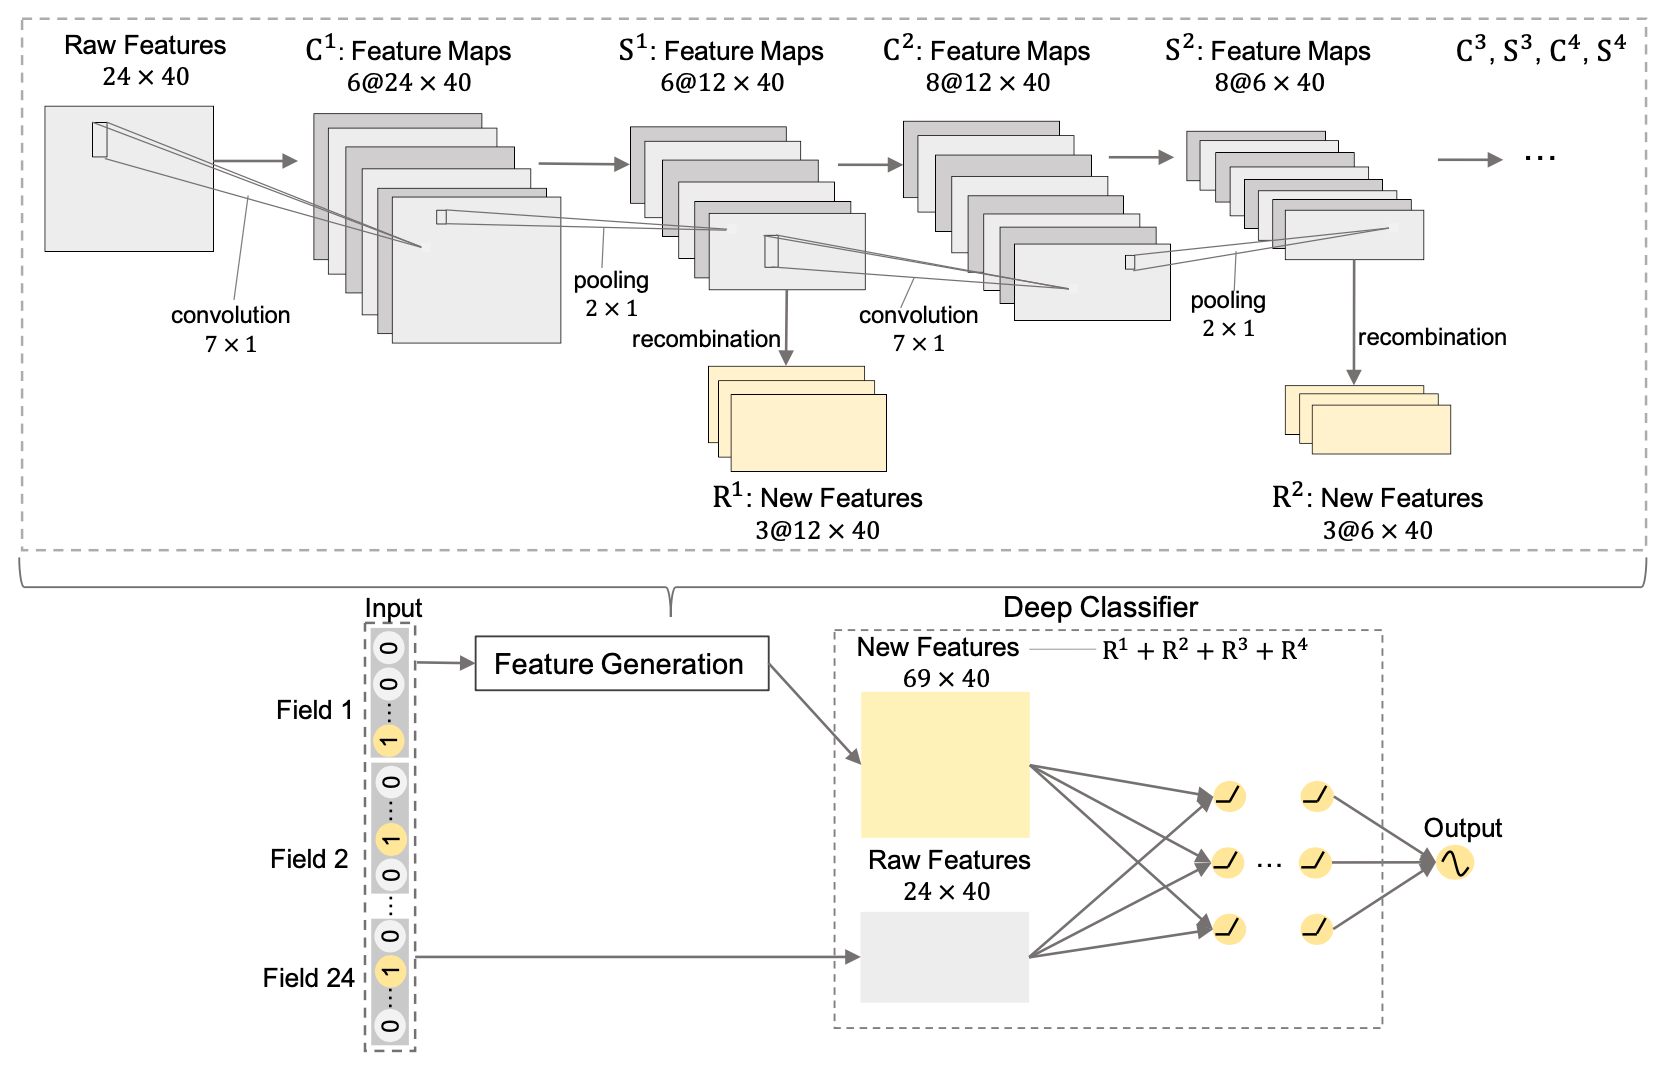
\includegraphics[width=.95\linewidth]{FGCNN}
  \caption{FGCNN 模型总览}
  \label{fig:fgcnn}
\end{figure}

如图 \ref{fig:fgcnn} 所示,FGCNN 由特征生成器和深度分类器组成,其中深度分类器就是指某个现成的 CTR 模型,比如 PNN 或者 DeepFM。
然后特征生成器主要就是 CNN 外加重组层。
首先值得一提的就是输出为 $e \in \mathbb{R}^{M \times D}$,FGCNN 把它看成通道数为 1 的一张 2D 图。
长为 $M$ 也就是域的数量,宽为 $D$ 也就是嵌入维度。
对于卷积层和池化层,他们的 filter 大小都是 $k \times 1$,也就是宽为 1。
这样整个过程中宽度是不变的,方便最后拼接到原嵌入表示去。
因为卷积和池化与正常的 CNN 无异,所以这里不展开说了。

在前面也提到过,CNN 只能学习到局部特征,而 CTR 的数据往往不看顺序,所以 FGCNN 还使用了重组层来学习全局特征。
全文大概最有意思的就是这个重组层了,其实重组层就是一个全连接层,
只不过池化层输出为三维张量,我需要先把它展平成一维然后再用全连接层。
最后 FGCNN 把 CNN 中每一个池化的输出都用重组层提取一遍全局特征,然后再跟原特征拼在一起。
这就变成了深度 CTR 分类器的输入数据了。

\chapter{评价指标}
\label{chap:metrics}

对于评价指标,我使用两个指标来评估模型。AUC(ROC曲线下面积)和Logloss(交叉熵)。这两个指标评估来自两个不同方面的性能:

AUC衡量的是一个正向实例比随机选择的负向实例排名更高的概率。它只考虑了预测实例的顺序,对类不平衡问题不敏感。而Logloss则是测量每个实例的预测分数和真实标签之间的距离。有时我们更依赖Logloss,因为我们需要使用预测的概率来估计排名策略的收益(通常调整为CTR×bid)。

\chapter{数据集}

数据集我使用的是一个大小为一百万的 criteo 数据集 \footnote{\url{https://www.kaggle.com/leonerd/criteo-small}}, 老师给的那个数据集实在太小了,只有 10 万规模,很难满足训练需求, 或者说复现结果会跟原文差很多。
Criteo 原始数据集由 4500 万规模,太大了,而且网站已经 404 无法下载了,于是我就没有尝试原始数据集。
Criteo 数据集是一个著名的工业基准数据集,用于开发预测广告点击率的模型,并可公开访问。 给定一个用户和他正在访问的页面,目标是预测他将点击给定广告的概率。
不过里面的数据全都是脱敏处理了.


\chapter{复现流程}

\section{数据预处理}

为了跟老师提供的数据集格式一致,因为我从 Kaggle 下载的数据集是 txt 格式的,缺少表头和一些预处理。
所以我首先使用 kaggle-2014-criteo \footnote{\url{https://github.com/ycjuan/kaggle-2014-criteo}}提供的小工具,执行 \texttt{converters/txt2csv.py tr train\_1m.txt} j将数据预处理为 \texttt{csv} 格式。
并且对于每一列,列名以 C 开头的表示离散的类别特征,I 开头的为连续特征。
列名为 \texttt{Label} 的那一列就是标签。

首先将数据分为离散和连续两种,并且对 NaN 填充为 '-1' 和 0。
然后使用 scikit 提供的 LabelEncoder 将离散的类别标签(字符串)变为整数标签 id。
对于连续型数据,直接缩放到 $0 \sim 1$ 的范围。

我将数据集以 2020 为随机数种子,按照 $8 : 2$ 比例随机划分为训练集和测试集。
最后得到训练集 640000 个样本,测试集 160000 个样本。

代码如下:

  \begin{minted}[texcomments,tabsize=2,fontsize=\footnotesize,style=friendly,bgcolor=friendlybg]{python}
data = pd.read_csv('./criteo_small.csv'); target = ['Label']
# 按照列名分为离散和连续型
sparse_features = ['C' + str(i) for i in range(1, 27)]
dense_features = ['I' + str(i) for i in range(1, 14)]
# 数据清洗
data[sparse_features] = data[sparse_features].fillna('-1', )
data[dense_features] = data[dense_features].fillna(0, )
# 离散标签变为整数 id
for feat in sparse_features:
    lbe = LabelEncoder(); data[feat] = lbe.fit_transform(data[feat])
# 连续特征缩放到 0 ~ 1
mms = MinMaxScaler(feature_range=(0, 1))
data[dense_features] = mms.fit_transform(data[dense_features])
# 特征列的名称,DNN 和 线性都用相同的特征列,因为我们没有基于专家经验的特征组合
fixlen_feature_columns = [SparseFeat(
    feat, vocabulary_size=data[feat].nunique(),
    embedding_dim=4) for feat in sparse_features] + [DenseFeat(
    feat, 1, ) for feat in dense_features]
dnn_feature_columns, feature = [fixlen_feature_columns, ] * 2
# 划分训练和测试集
train, test = train_test_split(data, test_size=0.2, random_state=2020)
  \end{minted}

代码位于 \texttt{recommender.ipynb} 文件。

\section{模型的实现}

该网络主要由 Embedding,DNN 和 CIN 组成。下面将逐个组件得列出核心代码
还有最后 xDeepFM 负责把这些组件合在一起。
这些组件和对应的文件位置分别为:

\begin{enumerate}
  \item CIN: \texttt{layers/interactions.py}
  \item Embedding: \texttt{inputs.py}
  \item DNN: \texttt{layers.py}
  \item xDeepFM: \texttt{models/xdeepfm.py}
\end{enumerate}

\subsection{Embedding}

  \begin{minted}[texcomments,tabsize=2,fontsize=\footnotesize,style=friendly,bgcolor=friendlybg]{python}
def create_embedding_dict(sparse_feature_columns, seed, l2_reg,
                          prefix='sparse_'):
    sparse_embedding = {}
    # 离散数据,每一个 field 创建一个 embedding
    for feat in sparse_feature_columns:
        emb = Embedding(feat.vocabulary_size, feat.embedding_dim,
                        embeddings_initializer=feat.embeddings_initializer,
                        embeddings_regularizer=l2(l2_reg),
                        name=prefix + '_emb_' + feat.embedding_name)
        emb.trainable = feat.trainable
        sparse_embedding[feat.embedding_name] = emb
  \end{minted}

\subsection{DNN}


  \begin{minted}[texcomments,tabsize=2,fontsize=\footnotesize,style=friendly,bgcolor=friendlybg]{python}
class DNN(Layer):
    def __init__(self, hidden_units, l2_reg=0,
                 seed=1024, **kwargs):
        self.hidden_units = hidden_units
        self.l2_reg = l2_reg
        self.seed = seed
        super(DNN, self).__init__(**kwargs)

    def build(self, input_shape):
        input_size = input_shape[-1]
        hidden_units = [int(input_size)] + list(self.hidden_units)
        # 最主要的两个参数 W 和 b
        self.kernels = [self.add_weight(name='kernel' + str(i),
                                        shape=(
                                            hidden_units[i],
                                            hidden_units[i + 1]),
                                        initializer=glorot_normal(
                                            seed=self.seed),
                                        regularizer=l2(self.l2_reg),
                                        trainable=True) for i in range(len(
                                            self.hidden_units))]
        self.bias = [self.add_weight(name='bias' + str(i),
                                     shape=(self.hidden_units[i],),
                                     initializer=Zeros(),
                                     trainable=True) for i in range(len(
                                            self.hidden_units))]
        super(DNN, self).build(input_shape)

    def call(self, inputs, training=None, **kwargs):
        deep_input = inputs
        # 简单的 MLP 的前馈计算
        for i in range(len(self.hidden_units)):
            fc = tf.nn.bias_add(tf.tensordot(
                deep_input, self.kernels[i], axes=(-1, 0)), self.bias[i])
            if self.use_bn:
                fc = self.bn_layers[i](fc, training=training)
            fc = self.activation_layers[i](fc)
            fc = self.dropout_layers[i](fc, training=training)
            deep_input = fc
        return deep_input
  \end{minted}

\subsection{CIN}

  \begin{minted}[texcomments,tabsize=2,fontsize=\footnotesize,style=friendly,bgcolor=friendlybg]{python}
class CIN(Layer):
    def __init__(self, layer_size=(128, 128), l2_reg=1e-5, seed=1024, **kwargs):
        self.layer_size = layer_size
        self.split_half = split_half; self.l2_reg = l2_reg; self.seed = seed
        super(CIN, self).__init__(**kwargs)

    def build(self, input_shape):
        self.field_nums = [int(input_shape[1])]
        self.filters = []; self.bias = []
        # 一堆参数
        for i, size in enumerate(self.layer_size):
            self.filters.append(self.add_weight(
                name='filter' + str(i),
                shape=[1, self.field_nums[-1]
                       * self.field_nums[0], size],
                dtype=tf.float32, initializer=glorot_uniform(
                    seed=self.seed + i),
                regularizer=l2(self.l2_reg)))
            self.bias.append(self.add_weight(
                name='bias' + str(i), shape=[size], dtype=tf.float32,
                initializer=tf.keras.initializers.Zeros()))
            self.field_nums.append(size)
        self.activation_layers = [activation_layer(
            self.activation) for _ in self.layer_size]
        super(CIN, self).build(input_shape)

    def call(self, inputs, **kwargs):
        dim = int(inputs.get_shape()[-1])
        hidden_nn_layers = [inputs]; final_result = []
        split_tensor0 = tf.split(hidden_nn_layers[0], dim * [1], 2)
        # 计算(核心就是reshape然后卷积):$X^k_{h,*} = \sum_{i=1}^{H_{k-1}} \sum_{j=1}^{M} W_{ij}^{k,h}(X_{i,*}^{k-1} \odot X_{j,*}^0)$
        for idx, layer_size in enumerate(self.layer_size):
            split_tensor = tf.split(hidden_nn_layers[-1], dim * [1], 2)
            dot_result_m = tf.matmul(split_tensor0, split_tensor, transpose_b=True)
            dot_result_o = tf.reshape(
                dot_result_m, shape=[dim, -1, self.field_nums[0] * self.field_nums[idx]])
            dot_result = tf.transpose(dot_result_o, perm=[1, 0, 2])
            curr_out = tf.nn.conv1d(
                dot_result, filters=self.filters[idx], stride=1, padding='VALID')
            curr_out = tf.nn.bias_add(curr_out, self.bias[idx])
            curr_out = self.activation_layers[idx](curr_out)
            curr_out = tf.transpose(curr_out, perm=[0, 2, 1])
            direct_connect = curr_out; next_hidden = curr_out
            final_result.append(direct_connect); hidden_nn_layers.append(next_hidden)
        result = tf.concat(final_result, axis=1)
        result = reduce_sum(result, -1, keep_dims=False); return result
  \end{minted}

\subsection{xDeepFM}

\
  \begin{minted}[texcomments,tabsize=2,fontsize=\footnotesize,style=friendly,bgcolor=friendlybg]{python}
def xDeepFM(linear_feature_columns, dnn_feature_columns, dnn_hidden_units=(256, 256),
            cin_layer_size=(128, 128,), l2_reg_linear=0.00001,
            l2_reg_embedding=0.00001, l2_reg_dnn=0, l2_reg_cin=0, seed=1024):
    features = build_input_features(
        linear_feature_columns + dnn_feature_columns)
    inputs_list = list(features.values())
    # 线性模型部分
    linear_logit = get_linear_logit(features, linear_feature_columns, seed=seed,
        prefix='linear', l2_reg=l2_reg_linear)
    # 嵌入层
    sparse_embedding_list, dense_value_list = input_from_feature_columns(features,
        dnn_feature_columns, 2_reg_embedding, seed)
    fm_input = concat_func(sparse_embedding_list, axis=1)
    dnn_input = combined_dnn_input(sparse_embedding_list, dense_value_list)
    # DNN 部分
    dnn_output = DNN(dnn_hidden_units, l2_reg_dnn,
        dnn_use_bn, seed=seed)(dnn_input)
    dnn_logit = tf.keras.layers.Dense(
        1,
        kernel_initializer=tf.keras.initializers.glorot_normal(seed))(dnn_output)
    final_logit = add_func([linear_logit, dnn_logit])
    # CIN 部分
    exFM_out = CIN(cin_layer_size,
                   l2_reg_cin, seed)(fm_input)
    # 加一个线性变换
    exFM_logit = tf.keras.layers.Dense(1,
        kernel_initializer=tf.keras.initializers.glorot_normal(seed))(exFM_out)
    final_logit = add_func([final_logit, exFM_logit])
    # 最后一个 affine 变换然后送到 sigmoid 输出为 0~1概率
    output = PredictionLayer(task)(final_logit)
    model = tf.keras.models.Model(inputs=inputs_list, outputs=output)
    return model
  \end{minted}

section{参数说明}

主要使用了以下参数

\begin{enumerate}
  \item lr:学习率
  \item EarlyStopping patience, 最多容忍 patience 代,训练的时候 loss 没下降,否则提前结束训练
  \item l2\_reg\_linear,线性模型部分的 L2 正则
  \item l2\_reg\_embedding, 嵌入层的 L2 正则
  \item l2\_reg\_dnn, DNN 部分的 L2 正则
  \item dnn\_hidden\_units, DNN 部分的层数以及隐藏单元的维度
  \item cin\_layer\_size, CIN 部分的层数以及隐藏单元的维度
  \item gpus, 使用的 GPU 数量
  \item train\_batch\_size, 训练的 batch 大小
  \item epochs, 最多训练代数
  \item validation\_split, 对训练机再划分出一定比例作为验证集
  \item test\_batch\_size, 测试时的 batch 大小
\end{enumerate}

\section{训练过程}
训练过程中使用到了以下几个参数:

\begin{enumerate}
  \item lr:设置为 $10^{-4}$
  \item EarlyStopping patience, 0
  \item l2\_reg\_linear,$10^{-3}$
  \item l2\_reg\_embedding, $10^{-3}$
  \item l2\_reg\_dnn, $10^{-3}$
  \item dnn\_hidden\_units, (400, 400)
  \item cin\_layer\_size, (200, 200)
  \item gpus, 3
  \item train\_batch\_size, 10240
  \item epochs, 200
  \item validation\_split, 0.2
\end{enumerate}

代码如下:

  \begin{minted}[texcomments,tabsize=2,fontsize=\footnotesize,style=friendly,bgcolor=friendlybg]{python}
tf.keras.backend.clear_session()
model_xdeepfm = xDeepFM(linear_feature_columns, dnn_feature_columns, task='binary',
                        l2_reg_linear=1e-3, l2_reg_embedding=1e-3,
                        l2_reg_dnn=1e-3, dnn_hidden_units=(400,) * 2,
                        cin_layer_size=(200,) * 2)
# 多 gpu 训练
model_xdeepfm = multi_gpu_model(model_xdeepfm, gpus=3)
# 优化器
model_xdeepfm.compile(tf.keras.optimizers.Adam(lr), "binary_crossentropy",
              metrics=['binary_crossentropy'])
# 记录日志到 tensorboard
log_dir="logs/fit/xDeepFM/" + datetime.datetime.now().strftime("%Y%m%d-%H%M%S")
tensorboard_callback = tf.keras.callbacks.TensorBoard(log_dir=log_dir, histogram_freq=1)
# 训练
history = model_xdeepfm.fit(train_model_input, train[target].values,
                            batch_size=10240, epochs=200, verbose=2,
                            validation_split=0.2,
                            callbacks=[es, time_callback, tensorboard_callback])
  \end{minted}


代码位于 \texttt{recommender.ipynb} 文件。

\section{测试过程}

测试过程的参数:

\begin{enumerate}
  \item test\_batch\_size, 4096
\end{enumerate}

测试部分的代码如下:

  \begin{minted}[texcomments,tabsize=2,fontsize=\footnotesize,style=friendly,bgcolor=friendlybg]{python}
# 测试
pred_ans = model_xdeepfm.predict(test_model_input, batch_size=4096)
print("test LogLoss (xDeepFM)", round(log_loss(test[target].values, pred_ans), 4))
print("test AUC (xDeepFM)", round(roc_auc_score(test[target].values, pred_ans), 4))
  \end{minted}


代码位于 \texttt{recommender.ipynb} 文件。

\section{AutoInt 模型复现过程}
\label{sec:autoint_reproduce}

因为 AutoInt 的输入与 xDeepFM 一致,也是分为 DNN 部分和线性模型部分。
而且我们没有基于专家经验的特征组合,所以线性部分和 DNN 部分的输入都是一样的。

不过 DNN 部分除了 MLP 之外,就是多头自注意力网络了,也就是 InteractingLayer。
对于参数设置,因为使用的数据集太小,所以模型不能太大,而且训练过程中很容易过拟合。
所以对于多头注意力网络,使用很小的头(\texttt{att\_head\_num = 2})并且添加一些正则化项。
同时,使用较小的学习率 $lr = 10^{-4}$。

复现代码如下:


  \begin{minted}[texcomments,tabsize=2,fontsize=\footnotesize,style=friendly,bgcolor=friendlybg]{python}
# 因为要在同一个进程运行多个模型,所以要先清理以下之前的 tf 回话
tf.keras.backend.clear_session()
model_autoint = AutoInt(linear_feature_columns, dnn_feature_columns,
                        task='binary', l2_reg_linear=1e-5, att_layer_num=2,
                        l2_reg_embedding=1e-5,  l2_reg_dnn=1e-5, att_head_num=2,
                       )
model_autoint = multi_gpu_model(model_autoint, gpus=3)
model_autoint.compile(tf.keras.optimizers.Adam(1e-4), "binary_crossentropy",
                      metrics=['binary_crossentropy'], )
log_dir="logs/fit/AutoInt/" + datetime.datetime.now().strftime("%Y%m%d-%H%M%S")
tensorboard_callback = tf.keras.callbacks.TensorBoard(log_dir=log_dir, histogram_freq=1)
# 训练
history = model_autoint.fit(train_model_input, train[target].values,
                            batch_size=10240, epochs=200, verbose=2, validation_split=0.2,
                            callbacks=[es, time_callback, tensorboard_callback]
                           )
# 测试结果
pred_ans = model_autoint.predict(test_model_input, batch_size=4096)
print("test LogLoss (AutoInt)", round(log_loss(test[target].values, pred_ans), 4))
print("test AUC (AutoInt)", round(roc_auc_score(test[target].values, pred_ans), 4))
  \end{minted}

AutoInt 的实现代码与 xDeepFM 类似,相当于把 CIN 换成多头自注意力网络(InteractingLayer)。
InteractingLayer 的具体实现见 \texttt{layers.interaction.py},基本上就是按照多头注意力的公式来,这里就不赘述了。

\section{FGCNN 复现流程}
\label{sec:fgcnn_reproduce}

FGCNN 可以立即为是一个自动特征生成器,它利用卷积和重组层学习到新的特征,于旧特征拼接在一起组成新特征。
再把这个新特征放进一个 CTR 分类器中去,这个分类器在论文中默认是 IPNN,当然也可以很简单的换成其他的模型。
FGCNN 的核心就是卷积和池化再加上重组(flatten + dense),具体的代码见 \texttt{interaction.py}。

对于超参数的设置,基本和 xDeepFM 类似,因为使用了三块 2080Ti,所以使用了很大的 batch size。
卷积核大小和池化层的 filter 大小真的好难调出满意的。

复现流程的代码如下:

  \begin{minted}[texcomments,tabsize=2,fontsize=\footnotesize,style=friendly,bgcolor=friendlybg]{python}
tf.keras.backend.clear_session()
model_fgcnn = FGCNN(linear_feature_columns, dnn_feature_columns,
                    task='binary', l2_reg_linear=1e-4, l2_reg_embedding=1e-4,
                    l2_reg_dnn=1e-4, conv_kernel_width=(9,) * 2, pooling_width=(2,)*2,
                    dnn_hidden_units=(1024, 1), new_maps=(3,) * 2,
                    conv_filters=(38, 40))
model_fgcnn = multi_gpu_model(model_fgcnn, gpus=3)
model_fgcnn.compile(tf.keras.optimizers.Adam(0.00001), "binary_crossentropy",
                   metrics=['binary_crossentropy'])
log_dir="logs/fit/FGCNN/" + datetime.datetime.now().strftime("%Y%m%d-%H%M%S")
tensorboard_callback = tf.keras.callbacks.TensorBoard(log_dir=log_dir, histogram_freq=1)
# 训练
history = model_fgcnn.fit(train_model_input, train[target].values,
                         batch_size=10240, epochs=200, verbose=2, validation_split=0.2,
                         callbacks=[es, time_callback, tensorboard_callback])
# 测试结果
pred_ans = model_fgcnn.predict(test_model_input, batch_size=4096)
print("test LogLoss (FGCNN)", round(log_loss(test[target].values, pred_ans), 4))
print("test AUC (FGCNN)", round(roc_auc_score(test[target].values, pred_ans), 4))
  \end{minted}

\chapter{实验结果及分析}
\label{chap:result}

\begin{figure}[h]
\centering%
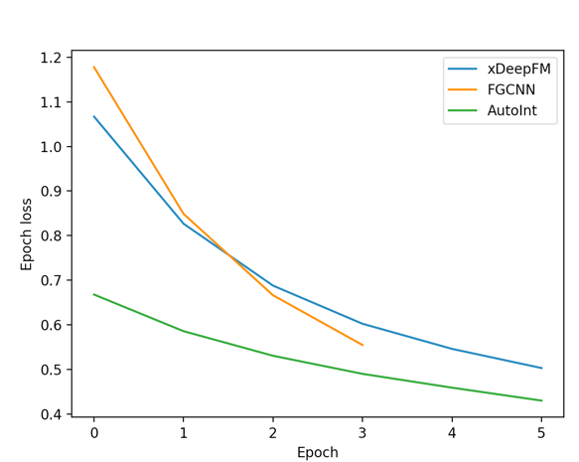
\includegraphics[width=.7\linewidth]{train_loss_ctr}
  \caption{训练集损失图}
  \label{fig:train_loss}
\end{figure}

\begin{figure}[h]
\centering%
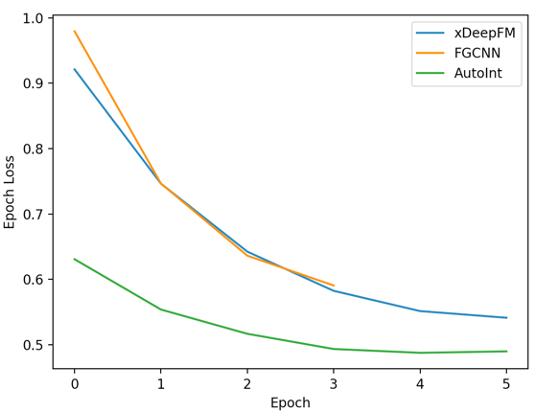
\includegraphics[width=.7\linewidth]{val_loss_ctr}
  \caption{验证集损失图}
  \label{fig:val_loss}
\end{figure}

xDeepFM, FGCNN 和 AutoInt 三种模型每一代的训练集和验证集上的损失值如图 \ref{fig:train_loss} 和 \ref{fig:val_loss} 所示。
损失值为交叉熵,在 CTR 领域中也称 \texttt{LogLoss},计算公式请参考公式 \ref{eq:loss}。
训练过程使用 EarlyStopping 避免浪费时间在过拟合上。
值得一提的是,因为使用的 batch 超级大(10240),使得训练过程虽然是 mini batch 随机梯度下降不过更加像全局梯度下降了,总是就是很快就收敛了。

\begin{table}[htb]
  \centering
  \caption{复现的测试集 AUC 结果以及原文结果对比}
  \label{tab:reproduce_auc}
  \begin{tabular}{ccc}
    \toprule
    \textbf{论文}         & \textbf{复现的 AUC}           & \textbf{原文结果 AUC}            \\
    \midrule
    \textbf{xDeepFM} (\cite{xdeepfm}) & 0.7574 & 0.8052 \\
    \textbf{FGCNN} (\cite{fgcnn})           & 0.737           & 0.8022  \\
    \textbf{AutoInt} (\cite{autoint})         & 0.7579           & 0.8061 \\
    \bottomrule
  \end{tabular}
\end{table}

对于测试阶段,使用的评价指标为 AUC(在第 \ref{chap:metrics} 章中介绍)。
最终取训练过程中验证集损失值最低的那一代的模型(也就是最后一代啦)用作测试。
复现出来的测试结果如表 \ref{tab:reproduce_auc} 所示。
从结果可以看出来,三种方法的复现的结果都低于原文的结果。
经过分析,我认为主要有以下几个原因:

\begin{itemize}
  \item 使用的数据集为 100 万规模的小数据集而不是 Criteo 原数据集的 4500 万规模,在数据集规模上差了 45 倍,很难发挥出模型的最佳性能。
  \item 因为数据集有变化,所以论文中使用的最优超级参数很可能已经不再适用,我自己也调了好久的超参数,也还没找到最满意的超参数。
  \item batch size 过大,这导致每一代的更新次数很少(10240 的 batch size 意味着每一代基本上只更新 60 多次),这样的优化结果肯定不如小火慢炖的 mini batch 随机梯度下降。
\end{itemize}

总的来说,复现结果还算令人满意,复现结果与论文的性能符合预期。
不过这里面的 FGCNN 复现结果差强人意,我认为原因有以下几个:

\begin{itemize}
  \item FGCNN 里面用的默认的分类器是 PNN,PNN 是很早起的工作了,结果当然不如 xDeepFM
  \item FGCNN 里面的核心--卷积的使用基本没多少道理,用卷积学习这些 fields 之间的局部特征就很扯淡。因为 Criteo 里面的 field 都是脱敏的,也就是说根本不知道这些 field 具体是什么,于是乎这些数据的顺序也是可以随意摆放的。如果把相近的 fields 放在一起还能解释一些这个局部特征。
  \item FGCNN 的卷积的超参数比较多,而且从论文中也可以看出来,作者花了大量的时间来调参数,而且每一个数据集他们公布的最优超参数都不一样。我用的论文给的 Criteo 的超参数大概率是不能用在我这个小数据集上的。
\end{itemize}

\begin{table}[htb]
  \centering
  \caption{时间复杂度测试}
  \label{tab:time_complex}
  \begin{tabular}{cc}
    \toprule
    \textbf{论文}         & \textbf{每一代花费的时间}  \\
    \midrule
    \textbf{xDeepFM} (\cite{xdeepfm}) & 7s \\
    \textbf{FGCNN} (\cite{fgcnn})           & 32s \\
    \textbf{AutoInt} (\cite{autoint})         & 6s \\
    \bottomrule
  \end{tabular}
\end{table}

此外,我还测试了这三种方法训练一代的时间花费,以此来反映模型的时间复杂度。
结果如表 \ref{tab:time_complex} 所示,可以发现一个有意思的事情。
FGCNN 的复杂度也太高了吧,三块 2080Ti 都顶不住!
而且结果还这么的离谱,就算是按照 FGCNN 论文中的那样,结果高于 xDeepFM 低于 AutoInt,那时间复杂度也直接被 AutoInt 吊打啊。
而且 AutoInt 用 3 层 2-头自注意力网络的情况下,速度还比用两层 CIN 的 xDeepFM 要好,说明 CIN 的时间复杂度也确实有点高。

\chapter{结论}

本文系统地介绍了推荐系统领域中点击率预测任务的发展情况以及主要方法论。
同时,详细介绍了 xDeepFM,AutoInt 和 FGCNN 这三篇论文的方法。
在 Criteo 数据集上的复现结果中发现了一些有意思的结论。
阅读了许多文献后,我发现,CTR 任务在评价标准(例如 AUC)上提升已经非常缓慢了。
不过已有的论文的时间复杂度过大在工业界部署的时候是一个重要的问题。
例如 xDeepFM 的 CIN,Deep \& Cross 的 Cross,虽然它们都能很好的学习显式的特征组合,可是他们带来的复杂度还是比较大的。
最近的论文,如 \cite{deeplight} 提出的 DeepLight 正在致力于解决这类问题,用牺牲很少一点的精度来换取大量的计算复杂度上的优化,在实际部署中是非常有意义的,这将是未来研究 CTR 的一个重要方向。
同时,AutoInt 这类论文也为学习高阶特征组合带来了更加复杂的神经网络的可能,已有的大量的基于 Transformer 的模型也许能派上用场。

\chapter{所完成的加分项}

\begin{table}[htb]
  \centering
  \caption{加分项统计}
  \label{tab:time_complex}
  \begin{tabular}{cc}
    \toprule
    \textbf{加分项目}         & \textbf{位置}  \\
    \midrule
    对 xDeepFM 之后的论文的文献综述 & 第 \ref{sec:after_xeepfm} 小节 \\
    对 xDeepFM 之后的论文的算法模块介绍           & 第 \ref{sec:autoint} 和 \ref{sec:fgcnn} 节 \\
    AutoInt 和 FGCNN 的复现过程        & 第 \ref{sec:autoint_reproduce} 和 \ref{sec:fgcnn_reproduce} 节 \\
    AutoInt 和 FGCNN 的复现结果和分析 & 第 \ref{chap:result} 章 \\
    \bottomrule
  \end{tabular}
\end{table}

% 其他部分
\backmatter

% 参考文献
\bibliography{ref/refs}  % 参考文献使用 BibTeX 编译

% 附录
\appendix

\chapter{文件清单}

\begin{table}[htb]
  \centering
  \caption{文件清单}
  \label{tab:files}
  \begin{tabular}{cc}
    \toprule
    \textbf{文件(夹)}         & \textbf{说明}  \\
    \midrule
    \texttt{report.pdf} & 课程报告 PDF 文件 \\
    \texttt{source/report}           & 课程报告 LaTeX 源文件 \\
    \texttt{source/recommender.ipynb}        & 数据预处理,训练和测试的代码 \\
    \texttt{source/code} & 实现模型的源代码 \\
    \bottomrule
  \end{tabular}
\end{table}

\begin{table}[htb]
  \centering
  \caption{模型实现代码文件清单(\texttt{source/code})}
  \label{tab:files}
  \begin{tabular}{cc}
    \toprule
    \textbf{文件}         & \textbf{说明}  \\
    \midrule
    \texttt{models/xdeepfm.py} & xDeepFM 实现代码 \\
    \texttt{models/fgcnn.py} & FGCNN 实现代码 \\
    \texttt{models/autoint.py} & autoint 实现代码 \\
    \texttt{layers/interacting.py}           & MLP (DNN) 和输出层 的实现 \\
    \texttt{layers/interacting.py}           & CIN, FGCNN, InteractingLayer 的实现 \\
    \texttt{layers/utils.py}        & 常用函数实现(e.g., softmax, reduce\_sum, 线性层) \\
    \texttt{feature\_column.py} & 离散特征和连续特征的抽象表示 \\
    \texttt{inputs.py} & 处理连续特征(变换)和离散特征(嵌入)\\
    \bottomrule
  \end{tabular}
\end{table}

\end{document}
